\documentclass[../main.tex]{subfiles}

\begin{document}

\section{Elementos sometidos axialmente a compresión}
\subsection{Ejercicio 1}

Determinar si la siguiente sección es: compacta, no compacta o con elementos 
esbeltos. Perfil W12x50, Acero F-36. 

\begin{figure}[ht]
  \centering
  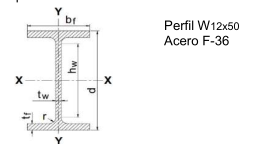
\includegraphics[width=0.4\textwidth]{../images/20210419/ej1}
  \caption{Perfil W12x50}
  \label{fig:ej1}
\end{figure}

Tomando de la tabla B.5.1, para el caso de las alas, consideramos lo siguiente:

\subsection{Alas de vigas laminadas}

Consideramos las alas como elementos no rigidizados. Tomamos el caso 1.
Encontramos el valor de $\lambda$ como:

\begin{align*}
  b * t 
.\end{align*}

Entrando a tabla de perfiles de CIRSOC, obtengo que:

\begin{align*}
  \frac{205*0.5}{16.3} = 6.28  
.\end{align*}

Y lo comparamos contra:

\begin{align*}
  0.56 * \sqrt{\frac{E}{F_y}} = 0.56 * \sqrt{\frac{210000}{355}} = 13.62  
.\end{align*}

Esto implica que \textbf{no es esbelto.}

\subsection{Alma de perfi}

Utilizamos el caso Nº12, con lo que llegamos a lo siguiente:

\begin{align*}
  \frac{h}{t_w} = \frac{241}{9.4} = 25.5
.\end{align*}

Y lo comparamos contra:

\begin{align*}
  1.49 * \sqrt{\frac{E}{F_y}} = 1.49 * \sqrt{\frac{200000}{355}} = 35.4
.\end{align*}

Vemos que \textbf{tampoco} esta pieza es esbelta.


\subsection{Ejercicio 2}
\textbf{Ver comentario para tipo de ejercicio sobre ejes.}

Para la estructura que se muestra en la siguiente imagen, se pide calcular la 
máxima carga última (Nu) que puede actuar en la COLUMNA N°3 perteneciente al Pórtico N°1. 

\begin{figure}[ht]
  \centering
  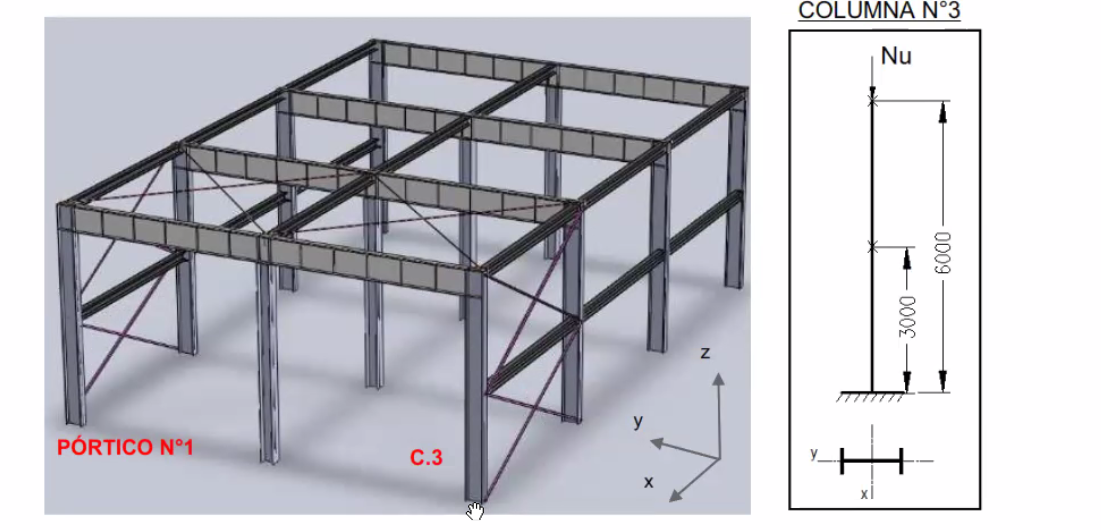
\includegraphics[width=0.8\textwidth]{../images/20210419/ej2}
  \label{fig:ej2}
\end{figure}

\begin{itemize}
  \item Sección de la columna laminado W12x50.
  \item Acero F-36.
  \item Base de la columna empotrada en el sentido desplazable del pórtico Nº1 y
    apoyada en la dirección perprendicular.
  \item Utilizar valores teóricos para el factor de longitud efectiva en ambas 
    direcciones, suponiendo para el sentido desplazable que la viga no aporta
    rigidez al giro en el extremo de la columna.
\end{itemize}

Lo primero que debemos encontrar es el valor de k. Luego, debemos encontrar el
valor de $\lambda_c$ como:

\begin{align*}
  \lambda_c = \frac{1}{\pi}*\frac{k*L}{r}*\sqrt{\frac{F_y}{E}} 
.\end{align*}

%Por último, a partir de este valor encontraremos el valor de $F_{cr}$.

\subsubsection{Dirección indesplazable}

Entrando a tabla, conseguimos que tenemos un factor de $k=1$. Con eso, obtenemos:

\begin{align*}
  \lambda_c = \frac{k*L}{r} = \frac{1*300}{4.98} * \frac{1}{\pi} * \sqrt{\frac{F_y}{E}}\\
  \lambda_c = 0.809
.\end{align*}

\subsubsection{Dirección desplazable}

Lo consideramos como empotrado libre, por lo que tenemos que considerar un $k=2$.
Entonces tenemos:

 \begin{align*}
  \lambda_c = \frac{2*600}{13.16} * \frac{1}{\pi} * \sqrt{\frac{255}{200000}} 
  \lambda_c = 1.22
.\end{align*}

Por lo tanto, adoptamos  $\lambda_c = 1.22$. Vemos también que  $\lambda_c \leq 1.5$,
por lo que podemos ultilizar lo siguiente:

\begin{align*}
  F_{cr} &= 0.658^{\lambda_c^{2}} * F_y \\
  F_{cr} &= 0.658^{1.22P^{2}} * 355 \\
  F_{cr} &= \SI{190}{MPa}
.\end{align*}

En caso de haber adoptado el otro, tendríamos un $F_{cr}= \SI{270}{MPa}$.

Podemos obtener la carga máxima de la siguiente forma:

\begin{align*}
  P_d &= \phi*P_n = \phi*F_{cr} * A \\
  P_d &= 0.85 * 190 * 94.84 * 10^{-1} \\
  P_d &= \SI{1531.6}{kN}
.\end{align*}

\subsection{Ejercicio 3}

\textbf{Ver comentario para tipo de ejercicio sobre ejes.}

Para la estructura que se muestra en la siguiente imagen, se pide calcular la
máxima carga última (Nu) de la columna indicada en la figura.

\begin{itemize}
  \item Sección de la columna IPB 300.
  \item Acero F-24.
  \item La base de la columna esta “empotrada” en el sentido desplazable y “apoyada” en la dirección
perpendicular.
\item Utilizar valores teóricos para el factor de longitud efectiva (k) en ambas direcciones, suponiendo
que, para el sentido desplazable, la viga no aporta rigidez al giro en el extremo de la columna.
\end{itemize}

\begin{figure}[htpb]
  \centering
  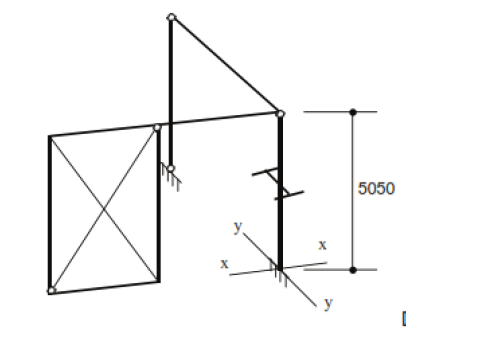
\includegraphics[width=0.8\textwidth]{../images/20210419/ej3}
  \caption{Diagrama ej 3}
  \label{fig:ej3}
\end{figure}

\subsubsection{Sentido indesplazable}

Es el dado en x-x. Para este caso, tenemos un caso caso artículado artículado,
por lo que k=1. Tenemos que la esbeltez será:

\begin{align*}
  \lambda = \frac{1*505}{7.58} = 66.62
.\end{align*}

\subsubsection{Sentido desplazable}

En este caso tenemos un empotrado libre, por lo que $k=2$. Entonces tenemos:

\begin{align*}
  \lambda = \frac{2*505}{13} = 77.7
.\end{align*}


\subsubsection{Calculo de $\lambda_c$}

Adoptamos el menor de ambos, por lo que:

\begin{align*}
  \lambda_c = \frac{1}{\pi} * 77.7 * \sqrt{\frac{235}{200000}} \\[5pt]
  \lambda_c = 0.848
\end{align*}

\subsubsection{Cálculo de $f_{cr}$}

Con el valor anterior, y viendo que $\lambda_c \leq 1.5$, tenemos:

\begin{align*}
  F_{cr} &= 0.658^{0,848^{2}}*235 \\[5pt]
  F_{cr} &= \SI{173.9}{MPa}
.\end{align*}

Con esto, obtenemos el valor de $N_u$ lo siguiente:

\begin{align*}
  N_u &= \phi * F_{cr} * A  \\[5pt]
  N_u &= 0.85 * 173.9 * 149 * 10^{-1} \\[5pt]
  N_u &= \SI{2202}{kN}
.\end{align*}

\end{document}
